\documentclass[11pt]{article}
\usepackage[margin=1in]{geometry}
\usepackage{graphicx}
\usepackage{amsmath, amssymb}
\usepackage{booktabs}
\usepackage{listings}
\usepackage{xcolor}
\usepackage{hyperref}
\usepackage{caption}
\usepackage{subcaption}
\usepackage{enumitem}

\definecolor{codebg}{RGB}{245,245,250}
\definecolor{cmdbg}{RGB}{40,42,54}
\definecolor{cmdfg}{RGB}{248,248,242}
\definecolor{kw}{RGB}{255,121,198}
\definecolor{str}{RGB}{241,250,140}

\lstdefinestyle{py}{
    language=Python,
    basicstyle=\ttfamily\small,
    backgroundcolor=\color{codebg},
    keywordstyle=\bfseries\color{blue!70!black},
    stringstyle=\color{green!50!black},
    commentstyle=\itshape\color{gray},
    breaklines=true, frame=single, framesep=4pt, showstringspaces=false}

\lstdefinestyle{shell}{
    language=bash,
    basicstyle=\ttfamily\footnotesize\color{cmdfg},
    backgroundcolor=\color{cmdbg},
    breaklines=true, frame=single, framesep=4pt, showstringspaces=false}

\hypersetup{colorlinks=true, urlcolor=blue, linkcolor=black,
            citecolor=black, breaklinks=true}

\title{\Large\bfseries triloop \& picoacq\\[2pt]
       \large User Manual and Documentation\\[8pt]
       \normalsize Three-loop magnetic-field array acquisition and analysis}
\author{}
\date{\today \\[6pt] \small Version 0.1.0}

\begin{document}
\maketitle

\tableofcontents
\bigskip\hrule\bigskip

%-----------------------------------------------------------------------
\section{Overview}
%-----------------------------------------------------------------------

\textsf{triloop} and \textsf{picoacq} are companion software packages
for HF radio polarimetry using three orthogonal magnetic-loop antennas:

\begin{itemize}\itemsep=2pt
\item \textsf{picoacq} drives a PicoScope 5444D (or any 5000-series)
      digitiser to capture three-channel coherent recordings, and
      writes them to a triloop-format HDF5 file.
\item \textsf{triloop} reads those files (or any compatible HDF5),
      extracts the narrow-band complex baseband at a target carrier,
      recovers the lab-frame magnetic field vector from the three loop
      measurements, and computes polarization-independent intensity,
      Stokes parameters, ellipticity, position angle, and a beamformed
      direction-of-arrival map.
\end{itemize}

The two packages share a common HDF5 file format
(Section~\ref{sec:fileformat}) so the analysis pipeline is independent
of the digitiser used for capture --- you can swap in a different
acquisition tool by writing the same file format.

\subsection{Audience}

This manual assumes basic Python familiarity (you can write
\texttt{import numpy as np} without looking it up), comfort with
command-line tools, and a working knowledge of complex baseband signal
processing.  Mathematical background on the cube-vertex array geometry
and polarimetry is covered in the companion technical report
\textsl{A Three-Loop Magnetic-Field Array for Polarization-Independent
HF Reception}; this manual focuses on \emph{using} the software.

\subsection{Quick start (five minutes)}

The most common workflow is a multi-band capture (all WWV bands at once
via bandpass undersampling at 15.625\,MS/s) followed by interactive
inspection of the resulting HDF5 file in a self-contained HTML browser:

\begin{lstlisting}[style=shell]
# Install
pip install -e ./triloop ./picoacq

# Make a synthetic capture (no hardware required) with all 5 WWV bands
picoacq capture -o cap.h5 --simulate \
    --sim-pol rcp --sim-faraday 30 --sim-snr 25

# Inspect metadata
triloop summary cap.h5

# Static QC plot (full-Nyquist PSD + per-band zooms + probe table)
triloop view cap.h5

# Interactive HTML browser (pan/zoom + animated polarization ellipse +
# intensity time history with fade CDFs)
triloop browse cap.h5

# Per-band scientific summary across all bands at once
triloop analyze-multi cap.h5 --az 9 --el 35
\end{lstlisting}

For the older single-band carrier workflow (when you only care about a
specific RF tone), use \texttt{triloop analyze} or
\texttt{triloop locate} — those still take \texttt{--carrier} explicitly
and operate directly on the captured baseband or IF signal.

%-----------------------------------------------------------------------
\section{Installation}
%-----------------------------------------------------------------------

Both packages are pure Python (with the optional exception of the
PicoScope SDK for hardware capture).  Recommended Python is 3.10 or
later.  Install both editable from the project tree:

\begin{lstlisting}[style=shell]
git clone <your-repo-url> triloop-project
cd triloop-project
pip install -e ./triloop          # analysis package
pip install -e ./picoacq          # acquisition package
\end{lstlisting}

\subsection*{Dependencies}
\begin{tabular}{lp{0.55\linewidth}}
\toprule
\textbf{Package} & \textbf{Why} \\\midrule
\texttt{numpy, scipy} & numerical core \\
\texttt{matplotlib} & figures \\
\texttt{h5py} & HDF5 read/write \\
\texttt{click} & command-line interface \\
\texttt{jupyterlab, ipywidgets} & (optional) for the analysis notebook\\
\texttt{picosdk} & (optional) PicoScope hardware support\\\bottomrule
\end{tabular}

For hardware capture you also need to install the PicoSDK system
library from \url{https://www.picotech.com/downloads}.  On macOS this
is a \texttt{.pkg} installer; on Linux it is a Debian \texttt{apt}
package or RPM; on Windows it is a regular installer.

\subsection*{Verifying installation}

After installation, the following two commands should each print a
short help message:
\begin{lstlisting}[style=shell]
triloop --help
picoacq --help
\end{lstlisting}

%-----------------------------------------------------------------------
\section{Coordinate systems and conventions}
\label{sec:conventions}
%-----------------------------------------------------------------------

\textsf{triloop} works in a right-handed Cartesian lab frame
$(E, N, \mathrm{Up})$.  Azimuth $\varphi$ is measured \emph{clockwise
from North} (so 0\textdegree\ is north, 90\textdegree\ is east).
Elevation $\theta$ is measured \emph{above the horizontal}.
A direction unit vector is

\begin{equation}
\hat{\mathbf{k}}(\varphi, \theta) =
\bigl(\cos\theta \sin\varphi,\;
      \cos\theta \cos\varphi,\;
      \sin\theta\bigr)^{\!\top}.
\end{equation}

\begin{figure}[h]\centering
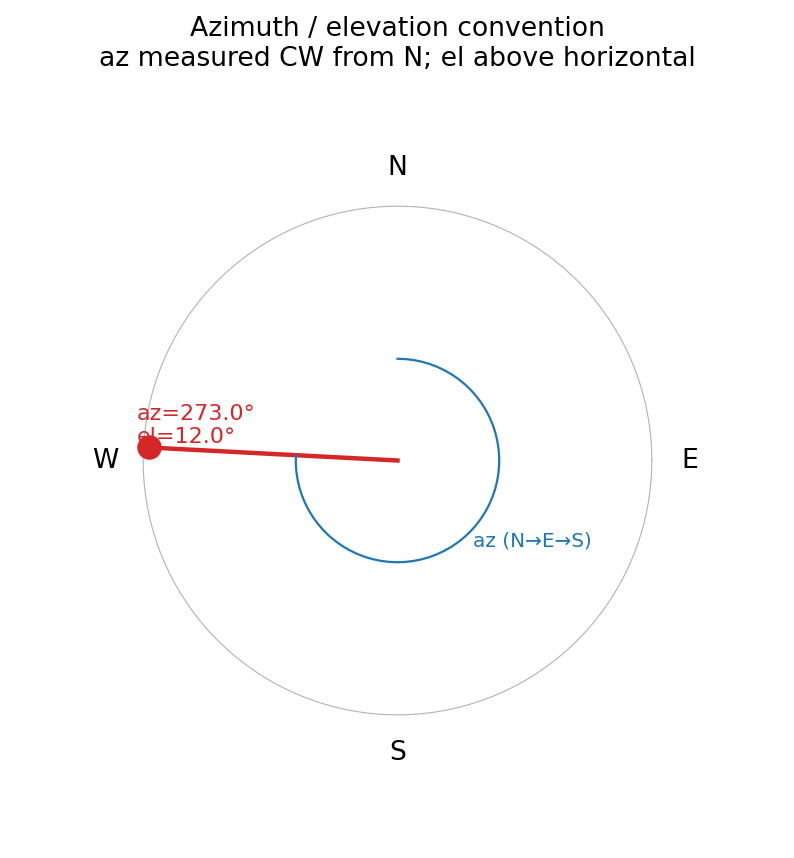
\includegraphics[width=0.55\linewidth]{figures/az_el_convention.png}
\caption{Azimuth/elevation convention used throughout
\textsf{triloop}.}\label{fig:azel}
\end{figure}

\subsection{The default cube-vertex layout}

\textsf{triloop}'s default geometry assumes the three loops sit on
three faces of a cube whose body diagonal is vertical and whose lower
vertex is on the ground (Figure~\ref{fig:cube}).  Each loop normal
tilts $35.26^\circ$ above the horizontal; their azimuthal projections
are spaced $120^\circ$ apart.  Loop \texttt{L1} points N$+$up, \texttt{L2}
points $+120^\circ$, \texttt{L3} points $-120^\circ$.

\begin{figure}[h]\centering
\begin{subfigure}[t]{0.45\linewidth}\centering
  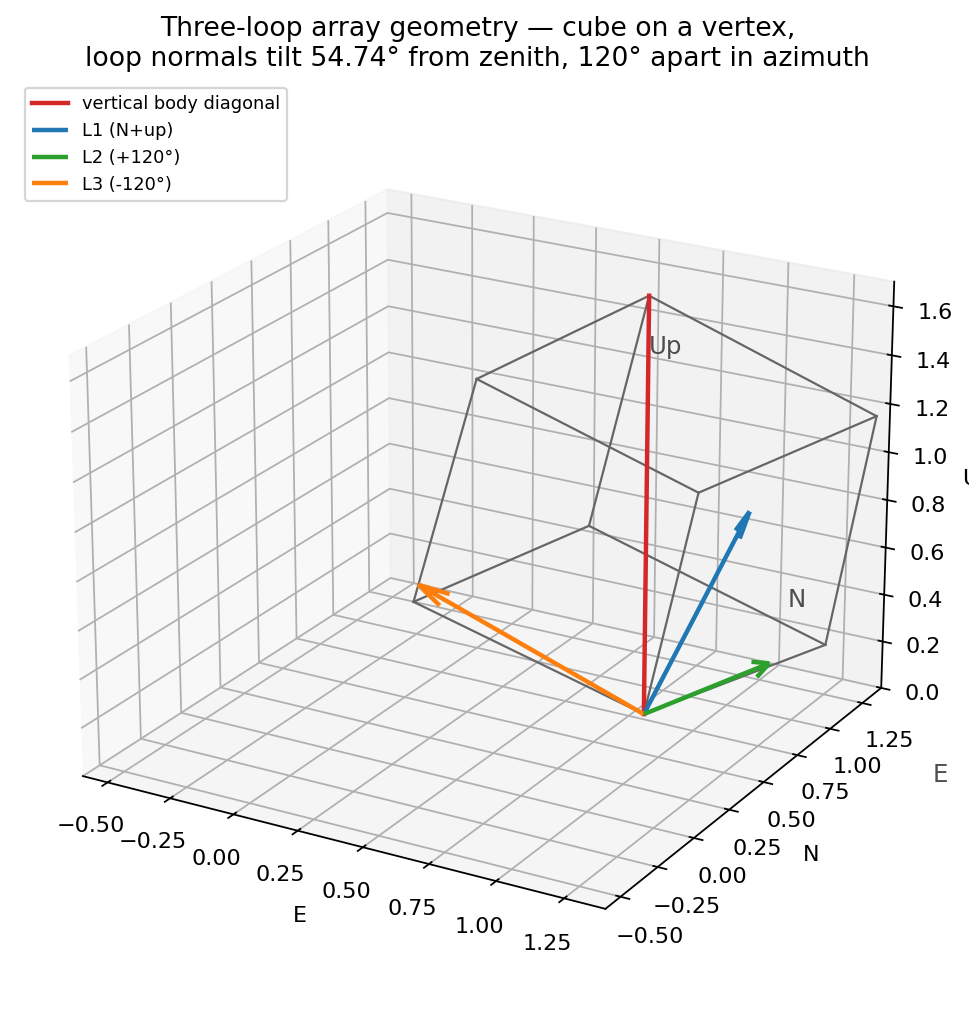
\includegraphics[width=\linewidth]{figures/geometry_cube.png}
  \caption{3-D view.}\label{fig:cube}
\end{subfigure}\hfill
\begin{subfigure}[t]{0.45\linewidth}\centering
  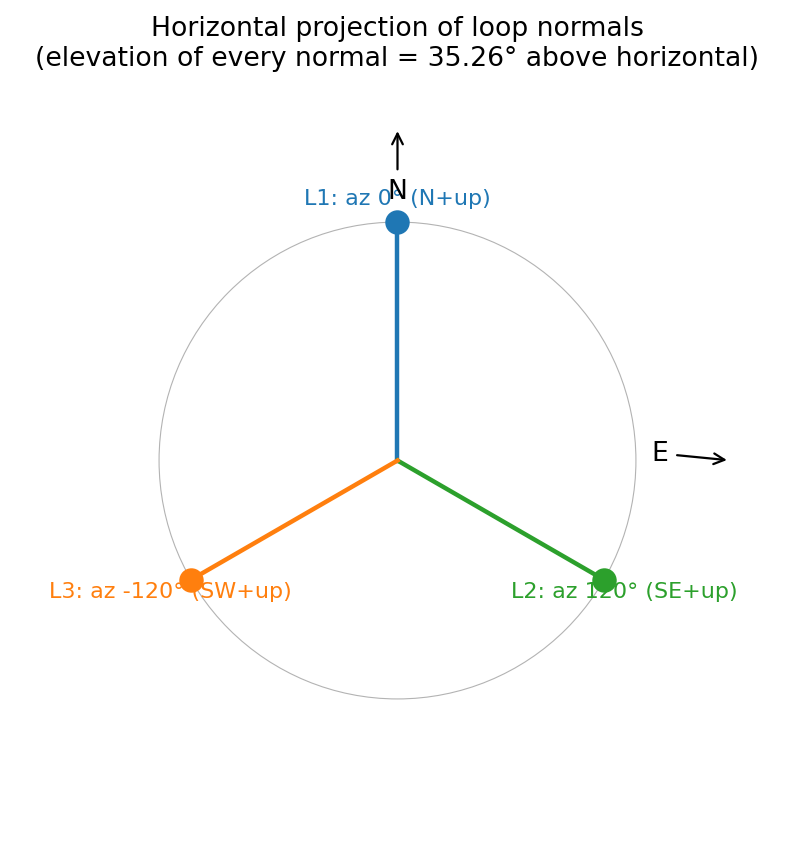
\includegraphics[width=\linewidth]{figures/normals_top_down.png}
  \caption{Top-down view.}\label{fig:topdown}
\end{subfigure}
\caption{Default loop geometry: cube on a vertex with body diagonal
vertical.  All three normals tilt $35.26^\circ$ above horizontal.}
\end{figure}

\subsection{Customising the loop geometry}
\label{sec:customising}

If your array does not match the default, you supply a different
\texttt{loops\_config} dict (in code) or edit it in the notebook.  The
schema:

\begin{lstlisting}[style=py]
loops_config = {
    "coordinate_frame":      "ENU",
    "azimuth_convention":    "cw_from_north",
    "elevation_convention":  "above_horizon",
    "loops": [
        {"name": "L1", "channel": "A",
         "normal_az_deg":   0.0,    # azimuth of loop normal, deg from N CW
         "normal_el_deg":  35.26,   # elevation of loop normal above horizontal
         "gain":            1.0,    # per-loop scalar gain calibration
         "phase_offset_deg": 0.0,   # per-loop electrical-phase calibration
        },
        {"name": "L2", "channel": "B", "normal_az_deg": 120.0, ...},
        {"name": "L3", "channel": "C", "normal_az_deg": -120.0, ...},
    ],
}
\end{lstlisting}

The \texttt{channel} field must match the channel names in the HDF5
capture (e.g.\ \texttt{"A"}, \texttt{"B"}, \texttt{"C"} for PicoScope
ports A, B, C).  Per-loop \texttt{gain} multiplies the corresponding
row of the geometry matrix \(\mathsf{N}\); \texttt{phase\_offset\_deg}
is applied to the complex baseband after extraction.

%-----------------------------------------------------------------------
\section{File format}
\label{sec:fileformat}
%-----------------------------------------------------------------------

Both \textsf{picoacq} and \textsf{triloop} use the same HDF5
v0.1 file format:

\begin{lstlisting}[style=shell]
/                          HDF5 root, attribute @format_version = "0.1"
/metadata                  group, with attributes:
    @sample_rate           float64, Hz
    @start_time_utc        ISO-8601 string
    @duration_s            float64
    @scope_model           string
    @scope_serial          string
    @capture_settings      JSON-encoded dict
    @loops_config          JSON-encoded dict
/channels                  group
    /A   ...               int16 or float32, length N
    /B
    /C
    /D                     optional reference channel
    Each channel dataset has attributes:
        @gain_v_per_count  float64
        @offset_v          float64
/time                      optional float64 dataset, length N
                           (regenerated from sample_rate if absent)
\end{lstlisting}

\textsf{triloop.io\_hdf5} provides \texttt{read\_capture()} and
\texttt{write\_capture()} which any third party can use to interoperate
with the toolchain.

%-----------------------------------------------------------------------
\section{The \texttt{picoacq} tool}
%-----------------------------------------------------------------------

\subsection{PicoScope 5444D hardware}
\label{sec:picohardware}

\textsf{picoacq} is written for the Pico Technology PicoScope 5444D
(``MSO,'' the variant with digital-channel breakout connectors, or the
non-MSO variants 5444B and 5444A which differ only in form factor).
Key properties relevant to coherent multi-channel acquisition:

\begin{itemize}\itemsep=2pt
\item \textbf{4 analog input channels} (BNC, switchable
      $1\,\mathrm{M\Omega}\,\|\,15$\,pF \emph{or} $50\,\Omega$).
\item \textbf{Variable-resolution ``FlexRes'' ADC} that operates from
      8 bits through 16 bits, with a corresponding sample-rate trade-off.
      For HF work in the operating mode \textsf{triloop} uses, the
      relevant point is \textbf{16-bit mode at 62.5\,MS/s on all four
      channels simultaneously}.
\item \textbf{Synchronous, time-aligned 4-channel sampling.}  All four
      channels share a single sample clock (one PLL) and a single
      trigger; channel-to-channel sample skew within a single capture
      is sub-picosecond (i.e.\ insignificant compared with any HF
      observable of interest).
\item \textbf{ADC architecture.}  The 5444D's FlexRes architecture
      can trade off bit-depth against per-channel sample rate, with
      the highest resolutions (15- and 16-bit) achieved by combining
      ADC cores via interleaving or pairing.  In the 16-bit
      four-channel mode that \textsf{triloop} uses, all four channels
      are produced as time-aligned sample streams; users requiring a
      definitive chip-level block diagram should consult the
      manufacturer's datasheet.  What matters for polarimetric work is
      that Pico specifies channel-to-channel sample skew below one
      sample period (i.e.\ $<\,16$\,ns at 62.5\,MS/s) and that this
      skew, plus any per-channel phase response of the analog
      front-end, is factory-calibrated and stored on the unit.
\item \textbf{Reference clock} can be switched between the internal
      PLL and an external 10\,MHz input, enabling phase-locked
      operation against a GPS-disciplined oscillator if required.
\item \textbf{Streaming over USB 3.0} sustainably at $\sim$\,400\,MB/s,
      enabling continuous capture at 62.5\,MS/s $\times$ 4 channels
      $\times$ 14-bit-packed.
\end{itemize}

\noindent\textbf{Coherence implication:} the four channels of a
5444D are sampled at the \emph{same instant} (within picoseconds), so
the channel-to-channel phase relations the analysis pipeline relies
on are preserved exactly.  Three of the four channels carry the
loop signals (\texttt{A}, \texttt{B}, \texttt{C}); the fourth
(\texttt{D}) is available for an optional reference such as a 1\,PPS
GPS pulse, a stable oscillator beacon, or simply unused.

\subsection{Software requirements}

To drive the scope from \textsf{picoacq} you need two things:

\begin{enumerate}\itemsep=2pt
\item The \textbf{PicoSDK system installer} from
      \url{https://www.picotech.com/downloads}.  This installs the
      shared library (\texttt{libps5000a.dylib} on macOS,
      \texttt{libps5000a.so} on Linux,
      \texttt{ps5000a.dll} on Windows) used to talk to the device.
\item The \texttt{picosdk} Python wrapper:
      \texttt{pip install picosdk} (or
      \texttt{pip install -e ./picoacq[hardware]}).
\end{enumerate}

\textsf{picoacq} accesses the PicoSDK via \texttt{ctypes}, configures
the scope into 16-bit four-channel block-acquisition mode, requests
the user's sample rate (selected by Pico's discrete \emph{timebase}
table; the closest available rate at or below the requested value is
used), and arms a software trigger.  After the block completes the
raw \texttt{int16} samples are pulled to host memory and converted to
volts using the per-channel range setting.

If the scope is not present or the SDK is missing, \textsf{picoacq}
prints a one-line warning and silently substitutes the simulator
described in Section~\ref{sec:simulator} so the rest of the analysis
toolchain can be tested without hardware.

\subsection{Field setup with PicoScope 7 (the GUI)}

Before driving the scope from \textsf{picoacq}, it is almost always
worth confirming the hardware works using Pico's free GUI application
\textbf{PicoScope 7} (\url{https://www.picotech.com/downloads}).
The macOS download is a regular \texttt{.dmg}; drag
\texttt{PicoScope.app} to \texttt{/Applications}.  The bundled
user-space USB plugin is authorised on first launch.

PicoScope 7 is the right tool for:

\begin{itemize}\itemsep=2pt
\item \textbf{First-light sanity check.}  Plug in the USB cable, launch
      PicoScope 7, enable channels A/B/C, and confirm you see live
      traces from each loop preamp.  This rules out cabling and driver
      issues before any code runs.
\item \textbf{Choosing voltage ranges.}  Watch the live time-domain
      trace to set each channel's $\pm$range so the strongest expected
      signal uses most of the dynamic range without clipping.  Pass
      those values to \texttt{picoacq capture --range\,\textit{V}}.
\item \textbf{Live FFT.}  PicoScope 7 has a built-in spectrum view.
      Confirm that the WWV or CHU carrier you are about to record is
      actually present (and at the expected detuned offset, e.g.\ near
      $2$\,kHz) before committing to a 60\,s capture.
\item \textbf{Noise floor.}  In spectrum view with the input
      terminated or the antenna disconnected, you can quickly verify
      your loop preamps aren't injecting birdies, oscillations, or
      excess broadband noise.
\item \textbf{Trigger setup.}  Edge / threshold / window triggers are
      easier to dial in interactively than via the SDK.  Once a useful
      configuration is found, replicate it in your \textsf{picoacq}
      command-line invocation.
\end{itemize}

PicoScope 7 holds an exclusive handle on the device while running, so
\textbf{quit PicoScope 7 before invoking \textsf{picoacq capture}}, or
the SDK call will fail with a ``device in use'' error.  Both
applications use the same factory calibration, so the channel-to-channel
phase relations measured in PicoScope 7 carry over to \textsf{picoacq}
captures.

\paragraph{Recommended workflow.}
\begin{enumerate}\itemsep=2pt
\item Install \texttt{PicoScope.app} from Pico's downloads page.
\item Plug the scope in via USB-3.  Authorise the kernel/user-space
      plugin on first launch when macOS prompts.
\item Connect loop preamps to channels A, B, C.
\item Use PicoScope 7 to set the voltage ranges and verify signal
      presence; record those ranges.
\item Quit PicoScope 7.
\item Install the PicoSDK system installer and the \texttt{picosdk}
      Python wrapper (Section~\ref{sec:picohardware}).
\item Run \texttt{picoacq capture} from the command line with the
      ranges you chose.
\end{enumerate}

\subsection{One-shot captures}

\begin{lstlisting}[style=shell]
# Default workflow: 8 s capture of all 5 WWV bands at once via
# bandpass undersampling at 15.625 MS/s, auto-ranged.
picoacq capture -o cap.h5             # all defaults

# Single-band IF capture (e.g. classical 200 kSPS audio-IF reception)
picoacq capture -o cap.h5 \
    --duration 60 --rate 200000 \
    --channels A,B,C --range 2.0 --no-auto-range \
    --rf-bands ""                     # disable rf_bands metadata
\end{lstlisting}

The default rate and \texttt{--rf-bands} setting in \textsf{picoacq}
are tuned for multi-band undersampling; see the \textit{picoacq User
Manual} for the band-to-baseband alias map and onboard-memory limits.

If the PicoSDK is not available or the scope is not connected,
\textsf{picoacq} prints a warning and falls back to the simulator
described in Section~\ref{sec:simulator}.

To force the simulator (e.g.\ on a laptop without hardware), pass
\texttt{--simulate} along with the simulation knobs:

\begin{lstlisting}[style=shell]
picoacq capture -o cap.h5 --simulate \
    --sim-pol     rcp \                 # or linear_vertical, lcp, ...
    --sim-faraday 30 \                  # deg/s Faraday rotation rate
    --sim-snr     25 \                  # per-channel SNR (dB)
    --sim-az      273 \
    --sim-el      12  \
    --sim-carrier 25000                 # IF carrier freq (Hz)
\end{lstlisting}

\subsection{Continuous monitoring}

For long-duration unattended runs, use \texttt{picoacq monitor}.  It
takes one capture every \texttt{--interval} seconds and writes a
timestamped file:

\begin{lstlisting}[style=shell]
picoacq monitor -d /data/triloop_runs/ \
    --interval 600 \                    # seconds between capture starts
    --duration 8 \                      # length of each capture (default)
    --prefix   wwv
# Stop with Ctrl-C, or pass --n-captures N to bound it.
\end{lstlisting}

The output filenames look like
\texttt{wwv\_20260520T144312Z.h5}.  SIGTERM and SIGINT are handled
cleanly --- the current capture finishes and the loop exits.

\subsection{The simulator}
\label{sec:simulator}

The simulator generates a synthetic three-loop dataset with controllable
arrival direction, polarization, additive Gaussian noise, and Faraday
rotation rate.  It is used both:
\begin{enumerate}\itemsep=2pt
\item by \texttt{picoacq capture --simulate} (and as the no-hardware
      fallback) to write a fully-formed HDF5 file with simulated data;
\item by \texttt{triloop simulate} to do the same thing without any
      acquisition driver in the loop.
\end{enumerate}

The polarization options are
\texttt{linear\_vertical, linear\_horizontal, rcp, lcp, elliptical}.
Faraday rotation rotates the polarization ellipse in the plane
perpendicular to $\hat{\mathbf k}$ at the specified rate; for
linearly-polarized input this produces classical Faraday fading on a
linear-pol receiver, while for circularly-polarized input it produces
no amplitude effect (just a common phase advance) --- a useful sanity
check.

%-----------------------------------------------------------------------
\section{The \texttt{triloop} tool}
%-----------------------------------------------------------------------

\subsection{Inspecting a capture}

\begin{lstlisting}[style=shell]
triloop summary cap.h5
\end{lstlisting}

prints something like:

\begin{lstlisting}[style=shell]
file:           cap.h5
format_version: 0.1
start_time_utc: 2026-05-20T14:43:12.345678+00:00
sample_rate:    200000 Hz
duration_s:     60 s
scope:          PicoScope 5444D (s/n EW123/4567)
channels:
  A: n=12000000, range=[-1.853, +1.967]
  B: n=12000000, range=[-1.732, +1.811]
  C: n=12000000, range=[-1.624, +1.703]
loops_config: 3 loops
\end{lstlisting}

\subsection{Single-file analysis}

\begin{lstlisting}[style=shell]
triloop analyze cap.h5 \
    --carrier 25000 \           # target carrier (Hz)
    --bw      2000 \            # analysis bandwidth (Hz, +/- BW/2 retained)
    --az      273 \             # initial guess azimuth (deg from N CW)
    --el      12  \             # initial guess elevation (deg above horizon)
    [--out summary.json]
\end{lstlisting}

The output is a JSON object on stdout (or written to \texttt{--out}):

\begin{lstlisting}[style=py]
{
  "input_file":             "/path/to/cap.h5",
  "sample_rate_Hz":         200000.0,
  "duration_s":             60.0,
  "f_peak_Hz":              25000.0954,
  "snr_db_per_loop":        [76.4, 76.5, 76.4],
  "az_initial_deg":         273.0,
  "el_initial_deg":         12.0,
  "median_pol_fraction":    1.0,
  "median_ellipticity_deg": -44.76,
  "median_position_angle_deg": 0.87,
  "instant_freq_mean_Hz":   25000.083,
  "intensity_mean":         0.99996,
  "intensity_std":          0.0109
}
\end{lstlisting}

\subsection{Direction finding (\texttt{triloop locate})}
\label{sec:locate}

The \texttt{analyze} command requires the user to supply an initial
$(\varphi, \theta)$ guess, which it then uses for the perp-plane
projection.  When the source direction is unknown, or when you want
the \emph{sharpest possible} direction estimate, use
\texttt{triloop locate} instead:

\begin{lstlisting}[style=shell]
triloop locate cap.h5 \
    --carrier 25000 --bw 2000 \
    --az0 270 --el0 15 \                # initial guess for the null sweep
    --half-width 30 --n-points 81 \     # local sweep grid
    --out-png residual_map.png          # optional residual heat-map
\end{lstlisting}

The pipeline is:

\begin{enumerate}\itemsep=2pt
\item Extract per-loop complex baseband at the carrier (same as
      \texttt{analyze}).
\item Form the lab-frame 3-vector $\mathbf z_{\rm lab}(t) = \mathsf{N}^{-1}\mathbf z_{\rm loops}(t)$
      and compute the $3\times 3$ coherency matrix
      $\mathsf{C} = \langle \mathbf z_{\rm lab}\mathbf z_{\rm lab}^H\rangle$.
\item \textbf{Eigendecomposition.}  The smallest-eigenvalue
      eigenvector of $\mathsf{C}$ is $\pm\hat{\mathbf k}_{\rm true}$
      (modulo the front/back ambiguity and the polarization
      degeneracy described in Section~\ref{sec:rank1}).  This gives
      the \emph{coarse} direction estimate.
\item \textbf{Null sweep.}  A 2-D grid of trial directions around
      that estimate (or around the user's \texttt{--az0/--el0}, if
      supplied) is searched to minimise the perp-residual energy
      $\langle |\hat{\mathbf k}_{\mathrm{trial}}\cdot\mathbf z_{\rm lab}|^2\rangle$.
      A parabolic fit on the $3\!\times\!3$ neighbourhood of the
      grid minimum yields a sub-grid direction.
\item The locked $(\hat{\mathbf k}_{\rm locked})$ is then used to
      project, recover the polarization basis, and compute the
      Stokes parameters and intensity (same as \texttt{analyze}).
\end{enumerate}

Why this works better than maximizing the directional response:
finding a maximum places you on a shallow plateau of $\cos^2\beta$,
while finding a null places you on the steep slope of $\sin^2\beta
\sim \beta^2$.  In typical conditions the null can be located $\sim
10\times$ more precisely than the response maximum, with the residual
sometimes 40\,dB or more below its peak.

\begin{figure}[h]\centering
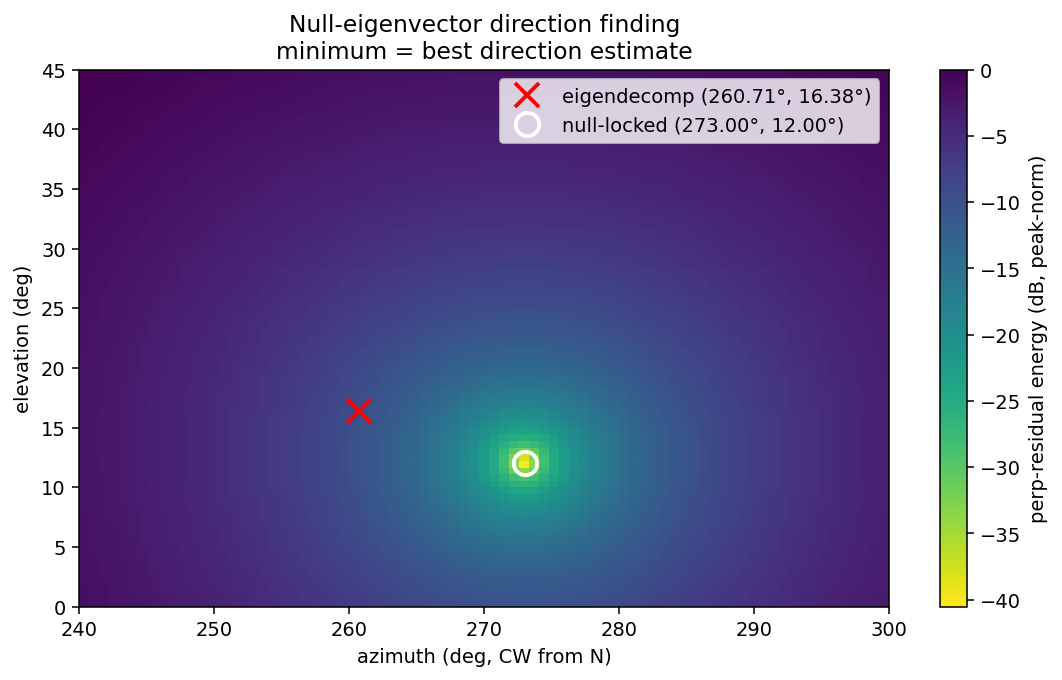
\includegraphics[width=0.7\linewidth]{figures/locate_demo_rcp.png}
\caption{Output of \texttt{triloop locate} on a high-SNR RCP
synthetic capture.  The eigendecomp seed (red \texttt{x}) was
displaced $\sim 12^\circ$ in azimuth from truth (273$^\circ$,
12$^\circ$); the null sweep refined it to $(272.998^\circ,
12.002^\circ)$, sub-$0.01^\circ$ accuracy.  Residual depth at the
locked direction is 40\,dB below the off-axis maximum --- this is
the ``software null'' equivalent of rotating a direction-finding
loop by hand.}
\label{fig:locate}
\end{figure}

The Python API mirrors the CLI:
\begin{lstlisting}[style=py]
from triloop import lock_and_analyze, read_capture
cap = read_capture("cap.h5")
res = lock_and_analyze(cap["time"],
                        cap["channels"]["A"], cap["channels"]["B"],
                        cap["channels"]["C"],
                        f0=25e3, BW=2e3,
                        az0=270, el0=15,
                        half_width_deg=30, n_points=81)
print(f"locked direction: az={res['az_locked']:.3f}°, "
      f"el={res['el_locked']:.3f}°")
print(f"null strength:   {res['eig']['null_strength']:.2e}")
\end{lstlisting}

\paragraph{When NOT to use \texttt{locate}.}  For purely linearly
polarized signals from a single station, the rank-1 coherency leaves
the direction ambiguous along an entire plane (Section~\ref{sec:rank1}).
\texttt{triloop locate} will return \emph{a} direction --- the one
with the smallest residual on its grid --- but that direction has no
physical meaning.  Use one of the rank-2-restoring conditions
(circular pol, Faraday rotation, multi-station triangulation) for
trustworthy localisation.

\subsection{Batch analysis}

\begin{lstlisting}[style=shell]
triloop batch /path/to/captures/ \
    --carrier 25000 --bw 2000 --az 273 --el 12 \
    --pattern '*.h5' \
    [--workers 4] \
    [--out triloop_batch_summary.jsonl]
\end{lstlisting}

writes one JSON line per capture into a single \texttt{.jsonl} file
(default: \texttt{triloop\_batch\_summary.jsonl} alongside the inputs).
This loads cleanly into pandas:

\begin{lstlisting}[style=py]
import pandas as pd
df = pd.read_json("triloop_batch_summary.jsonl", lines=True)
df["t"] = pd.to_datetime(df["start_time_utc"])
df.plot(x="t", y="median_ellipticity_deg")
\end{lstlisting}

\subsection{Multi-band analysis (\texttt{triloop analyze-multi})}
\label{sec:multiband}

When the capture file was produced by \texttt{picoacq} at the default
15.625\,MS/s rate, every WWV band (2.5, 5, 10, 15, 20\,MHz) is present
in a single recording at a different baseband alias position
(see the \textit{picoacq} manual, \S Default rate).
\texttt{analyze-multi} runs the full polarimetry pipeline once per
band, in a single command, and produces both a JSON-per-band summary
and a 5$\times$4 comparison plot:

\begin{lstlisting}[style=shell]
triloop analyze-multi cap.h5 --az 9 --el 35 \
    [--bw 4000] [--decim 20000] \
    [--rf-bands "2.5e6,5e6,10e6,15e6,20e6"] \
    [--loops-channels A,B,C] \
    [--out-png cap_multiband.png] \
    [--out-json cap_multiband.json]
\end{lstlisting}

The list of RF bands is read from the file's
\texttt{capture\_settings/rf\_bands\_hz} field by default; pass
\texttt{--rf-bands} only to override or restrict the set.  Each band's
baseband location is computed via
\texttt{picoacq.alias.alias\_of(rf, sample\_rate)}; even-Nyquist-zone
bands are conjugated so their analysis spectra read in the correct
frequency sense (see the \textit{picoacq} manual).

For each band the pipeline does:
\begin{enumerate}\itemsep=2pt
\item Brick-wall mix-and-LPF the real signal of every selected channel
      down to a complex baseband centred on the band's alias frequency,
      keeping $\pm$\texttt{bw}/2 of bandwidth.
\item Decimate to roughly \texttt{decim\_rate\_hz} (default 20\,kHz),
      which keeps phase information intact at the carrier scale of
      interest while shrinking arrays by 3 orders of magnitude.
\item Run \texttt{analyze\_z\_loops()} on the resulting (3, $N$)
      complex baseband matrix, exactly as
      \texttt{analyze} would on directly-mixed data.
\end{enumerate}

The output JSON has one record per band:

\begin{lstlisting}[style=py]
{
  "input_file": "...",
  "az_deg": 9.0, "el_deg": 35.0,
  "bw_hz": 4000.0, "decim_rate_hz": 20000.0,
  "loops_channels": ["A", "B", "C"],
  "bands": [
    {"rf_hz": 2500000.0, "baseband_hz": 2500000.0,
     "nyquist_zone": 1, "inverted": false,
     "snr_db_per_loop": [88, 89, 89],
     "median_pol_fraction": 1.0,
     "median_ellipticity_deg": 0.1,
     "median_position_angle_deg": 0.4,
     "intensity_mean": 1.0, "intensity_std": 0.02,
     "instant_freq_mean_Hz": 2500000.0},
    ...
  ]
}
\end{lstlisting}

Each band's row in the comparison PNG shows: intensity time series,
instantaneous-frequency residual, ellipticity (deg), and polarization
fraction.

\subsection{Quick-look QC (\texttt{triloop view})}
\label{sec:view}

\texttt{triloop view} produces a single static PNG for fast eyeballing:

\begin{lstlisting}[style=shell]
triloop view cap.h5 [--out-png cap_view.png] [--bw 8000]
\end{lstlisting}

Layout (top to bottom): full-Nyquist PSD with all channels overlaid and
each RF band annotated at its baseband alias position; per-band PSD
zooms (axis flipped for inverted/even-zone bands so frequencies read
correctly); a decimated time-domain trace of all channels; and the
auto-range probe table from
\texttt{capture\_settings/auto\_range\_probe} (peak / RMS / chosen
PicoScope range per channel).  This is the right tool to confirm
``did the capture work?'' before doing any heavier analysis.

\subsection{Magnetoionic O/X mode separation}
\label{sec:magnetoionic}

For ionospheric work a more physical decomposition than receiver-frame
Stokes parameters is the projection onto the propagation eigenmodes of
the magnetised plasma --- the \emph{ordinary} (O) and \emph{extraordinary}
(X) modes of Appleton-Hartree theory.  These modes are orthogonal and
their amplitude/phase are carried adiabatically from the ionosphere
exit point to the antenna with no further interaction (the medium is
gone), so they are the right basis for asking ``what came out of the
ionosphere?''.

\paragraph{Convention.} $\hat k$ is along the Poynting vector,
source $\to$ receiver.  $\theta$ is the angle between $\hat k$ and the
geomagnetic $\hat B$ at the relevant point.  $(\hat p_B, \hat q_B)$ is
the right-handed perpendicular-plane basis with $\hat p_B$ along the
projection of $\hat B$.  The Appleton-Hartree polarization parameter is
\[
\rho_{O,X}\;=\;\frac{E_{q_B}}{E_{p_B}}\;=\;-iq\;\pm\;i\sqrt{q^2+1},
\qquad q\;\equiv\;\frac{Y_T^2}{2\,Y_L\,(1-X)}
\]
with $Y = f_H/f$, $Y_L = Y\cos\theta$, $Y_T = Y\sin\theta$.  At the
exit point, $X = f_p^2/f^2 \to 0$ (the wave is leaving the plasma),
so the formula is a pure geometric calculation in $(\theta, f_H, f)$.

\paragraph{QL and QT regimes.}  At $\theta = 0$ (quasi-longitudinal,
$\hat k \parallel \hat B$), $Y_T = 0$ and $\rho_O \to +i$,
$\rho_X \to -i$ --- pure RCP/LCP about $\hat k$.  At $\theta = 90^\circ$
(quasi-transverse), $Y_L = 0$ and the modes degenerate to two
orthogonal linear polarizations along $\hat p_B$ and $\hat q_B$.  In
between, both modes are elliptical.  For most mid-latitude HF paths,
the descending exit-point $\theta$ falls in the 60--90$^\circ$ range
and the modes are moderately elliptical.

\paragraph{Computing the mode separation.}  Pass transmitter and
receiver coordinates to \texttt{analyze-multi}:

\begin{lstlisting}[style=shell]
triloop analyze-multi cap.h5 --az 9 --el 35 \
    --tx "40.6796,-105.0411" \    # Fort Collins WWV
    --rx "32.7803,-105.8200" \    # APO
    --reflection-height-km 250
\end{lstlisting}

Each band's JSON record then carries an additional
``\texttt{magnetoionic}'' field with the path geometry
($\theta$, $|B|$, $f_H$, exit-point lat/lon), the predicted mode
ellipticities, and the matched-filter outputs:
$\langle |a_O|\rangle$, $\langle |a_X|\rangle$,
$\langle |a_O|/|a_X|\rangle$, and
$\langle\Delta\varphi\rangle = \langle\arg a_O - \arg a_X\rangle$.

\paragraph{Faraday rotation.}  The total ``Faraday rotation'' that
would be seen on a single-linear-polarization receiver is the
path-integrated differential phase between the two modes,
\[
\Omega \;\approx\; \tfrac{e^3}{8\pi^2\varepsilon_0 m_e^2 c}\;
        \frac{\langle B\cos\theta\rangle\,\mathrm{TEC}}{f^2},
\]
provided by \texttt{triloop.integrated\_faraday\_rotation\_rad}.  At
30\,TECU on the FC$\to$APO path this is $\sim 4500$ turns at 2.5\,MHz
and $\sim 70$ turns at 20\,MHz.

\subsection{Worked paths: WWV $\to$ APO and WWV $\to$ Boston}
\label{sec:worked-paths}

The two tables below summarise the apparent angle of arrival and
the predicted O/X mode polarization at two reference receivers, both
listening to WWV's transmitter at Fort Collins, CO ($40.68^\circ$\,N,
$-105.04^\circ$\,W).  Reflection altitude is taken as 250\,km
throughout.  The fallback IGRF values are used for the geomagnetic
field; install \texttt{pyIGRF} for full IGRF-13 accuracy.

\paragraph{1.  FC $\to$ Apache Point Observatory  (APO, NM,
$32.78^\circ$\,N, $-105.82^\circ$\,W).}
880\,km path: a single F2 hop fits comfortably.  The path is nearly
N--S along the 105$^\circ$\,W meridian.

\begin{table}[h]\centering
\begin{tabular}{lc}
\toprule
\textbf{Path geometry} & \textbf{Value} \\\midrule
Great-circle range          & 881 km          \\
Hops                        & 1               \\
Reflection altitude         & 250 km          \\
\textbf{AoA elevation at RX (spherical Earth)} & \textbf{27.1$^\circ$} \\
AoA elevation at RX (flat Earth)               & 29.6$^\circ$ \\
\textbf{AoA azimuth at RX (great circle)}      & \textbf{4.3$^\circ$ from N CW} \\
Exit point lat / lon        & 34.76$^\circ$\,N, $-105.63^\circ$\,W \\
$\theta(\hat k, \hat B)$ at exit & 70$^\circ$       \\
$|B|$ at exit / $f_H$       & 50 µT / 1.40 MHz \\\bottomrule
\end{tabular}
\caption{FC $\to$ APO path geometry.}
\end{table}

\begin{table}[h]\centering
\begin{tabular}{ccccccl}
\toprule
$f$ (MHz) & $Y\!=\!f_H/f$ & $q$ & axial ratio & $\chi_O$ & $\chi_X$ & character \\\midrule
 2.5  & 0.56 & 0.71 & 0.52 & $+27^\circ$ & $-27^\circ$ & moderately linear \\
 5.0  & 0.28 & 0.35 & 0.71 & $+35^\circ$ & $-35^\circ$ & elliptical        \\
10.0  & 0.14 & 0.18 & 0.84 & $+40^\circ$ & $-40^\circ$ & elliptical        \\
15.0  & 0.09 & 0.12 & 0.89 & $+42^\circ$ & $-42^\circ$ & near-circular     \\
20.0  & 0.07 & 0.09 & 0.92 & $+43^\circ$ & $-43^\circ$ & near-circular     \\
\bottomrule
\end{tabular}
\caption{Mode polarization at the descending exit point for FC $\to$
APO. $Y \equiv f_H/f$, $q \equiv Y_T^2/(2 Y_L)$.  Both modes share
the same axial ratio; the X mode's major axis is rotated 90$^\circ$
from the O mode's (which lies along the projection of $\hat B$ onto
the perp-plane).}
\end{table}

\paragraph{2.  FC $\to$ Boston (Harvard, $42.37^\circ$\,N,
$-71.12^\circ$\,W).}
2812\,km path, well beyond the 1-hop F2 limit (~2200 km at low
elevation).  The dominant daytime mode is 2-hop F2 with a ground
bounce around Madison/Chicago.  The polarization that physically
arrives at Boston is set by the descending leg of the
\emph{last} hop (mid-bounce $\to$ Boston, ~1406 km).

\begin{table}[h]\centering
\begin{tabular}{lc}
\toprule
\textbf{Path geometry} & \textbf{Value} \\\midrule
Full great-circle range          & 2812 km            \\
Hops                             & 2 (last hop shown) \\
Last-hop range                   & 1406 km            \\
Reflection altitude              & 250 km             \\
\textbf{AoA elevation at RX (spherical Earth)} & \textbf{16.0$^\circ$} \\
AoA elevation at RX (flat Earth)               & 19.6$^\circ$ \\
\textbf{AoA azimuth at RX (great circle)}      & \textbf{277.7$^\circ$ from N CW} \\
Last-hop exit point lat / lon    & 42.48$^\circ$\,N, $-75.42^\circ$\,W \\
$\theta(\hat k, \hat B)$ at exit & 55$^\circ$         \\
$|B|$ at exit / $f_H$            & 50 µT / 1.40 MHz   \\\bottomrule
\end{tabular}
\caption{FC $\to$ Boston path geometry, last hop.}
\end{table}

\begin{table}[h]\centering
\begin{tabular}{ccccccl}
\toprule
$f$ (MHz) & $Y\!=\!f_H/f$ & $q$ & axial ratio & $\chi_O$ & $\chi_X$ & character \\\midrule
 2.5  & 0.56 & 0.33 & 0.72 & $+36^\circ$ & $-36^\circ$ & elliptical    \\
 5.0  & 0.28 & 0.16 & 0.85 & $+40^\circ$ & $-40^\circ$ & elliptical    \\
10.0  & 0.14 & 0.08 & 0.92 & $+43^\circ$ & $-43^\circ$ & near-circular \\
15.0  & 0.09 & 0.06 & 0.95 & $+43^\circ$ & $-43^\circ$ & near-circular \\
20.0  & 0.07 & 0.04 & 0.96 & $+44^\circ$ & $-44^\circ$ & near-circular \\
\bottomrule
\end{tabular}
\caption{Mode polarization at the descending exit point for the last
hop of FC $\to$ Boston.}
\end{table}

\paragraph{Key contrasts.}
\begin{itemize}\itemsep=2pt
\item Boston's last-hop $\theta = 55^\circ$ is closer to the QL limit
      than APO's $\theta = 70^\circ$, so at every band Boston's modes
      are \emph{more} circular than APO's.
\item Both paths show the same $f$-dependence: low frequency gives
      smaller axial ratio (more linear), high frequency gives larger
      axial ratio (more circular).  This is opposite to the
      Faraday-rotation magnitude, which is huge at low $f$ and small
      at high $f$.  ``Faraday large'' does \emph{not} mean ``modes
      circular'' --- the modes' shape and the path-integrated
      differential phase are independent observables.
\item The flat-Earth elevation overestimates the spherical-Earth
      elevation by 2.5--3.5$^\circ$ on these paths.  The
      \texttt{ExitGeometry} returned by
      \texttt{exit\_point\_geometry} carries both: use
      \texttt{el\_rx\_spherical\_deg} for operator-facing reports
      and antenna pointing.
\item The flat-Earth ``source bearing at RX'' that the code uses for
      its $\hat k$ direction is also slightly off compared to the
      proper great-circle initial bearing (1$^\circ$ for APO, 6$^\circ$
      for Boston).  The mode-polarization output uses the flat-Earth
      $\hat k$ for self-consistency with the rest of the geometry,
      but \texttt{az\_rx\_to\_src\_deg} reports the great-circle
      bearing for operator pointing.
\end{itemize}

\paragraph{Multi-hop paths.}  For paths beyond ~2200\,km, use the
\texttt{multi\_hop\_geometry} helper which returns the
\texttt{ExitGeometry} of the last hop:
\begin{lstlisting}[style=py]
from triloop import multi_hop_geometry
g = multi_hop_geometry(40.6796, -105.0411,    # FC
                       42.3744,  -71.1169,    # Boston
                       n_hops=2, h_km=250.0)
print(g.el_rx_spherical_deg, g.az_rx_to_src_deg, g.theta_deg)
\end{lstlisting}
For non-mid-latitude or non-symmetric paths (e.g.\ trans-equatorial
where the two hops have very different magnetic geometry) the
flat-mirror, equal-hop assumption breaks down and PHaRLAP-style
ray-tracing is the right tool.

\subsection{Interactive HTML browser (\texttt{triloop browse})}
\label{sec:browse}

\texttt{triloop browse} produces a self-contained HTML file (no
server, no external network — embeds Plotly via CDN) that lets you
pan, zoom, hover, and animate across the capture interactively:

\begin{lstlisting}[style=shell]
triloop browse cap.h5 \
    [--out-html cap_browse.html] \
    [--az 9 --el 35] \
    [--bw 4000] [--decim 20000] \
    [--n-anim-frames 60] \
    [--open-browser]
\end{lstlisting}

Layout: a tab bar at the top, with one ``Overview'' tab containing
the full-Nyquist PSD (channels toggle-able via the legend, RF-band
markers as dashed verticals), one ``Time series'' tab with decimated
time-domain traces, and one tab \emph{per RF band} containing four
panels:

\begin{enumerate}\itemsep=2pt
\item \textbf{PSD zoom} around the band centre (axis flipped for
      inverted bands).
\item \textbf{Intensity time history} with linear $|\mathbf{B}_\perp|^2$
      on the primary axis and dB-relative-median on a togglable
      secondary axis — useful for picking out fades.
\item \textbf{Intensity CDF} with P10 (10th-percentile) and P1
      (1st-percentile) fade-depth markers, the classical fade-margin
      metric for HF link-budget work.
\item \textbf{Animated polarization ellipse} drawn in the
      $(\mathrm{Re}\,A_p, \mathrm{Re}\,A_q)$ plane, with a
      Play/Pause control and a frame slider, so Faraday rotation
      and time-varying ellipticity become directly visible.
\end{enumerate}

The page is a single \texttt{.html} file you can email, version, scp,
or open in any modern browser.  No Python or server needed at
viewing time.

\subsection{Interactive analysis (Jupyter notebook)}

\begin{lstlisting}[style=shell]
triloop notebook cap.h5
\end{lstlisting}

opens the bundled analysis notebook with the file path pre-loaded.
The notebook has seven cells:

\begin{enumerate}\itemsep=2pt
\item \textbf{Load capture} --- reads metadata, prints summary.
\item \textbf{Loop geometry config} --- edit this cell to match your
      array (Section~\ref{sec:customising}).
\item \textbf{Analysis parameters} --- carrier, bandwidth, initial
      direction guess.
\item \textbf{Raw signals and spectra} --- 20 ms time-domain plot plus
      FFT power-spectra on all three loops.
\item \textbf{Run the pipeline} --- calls \texttt{analyze()} and prints
      summary statistics.
\item \textbf{Time-resolved diagnostics} --- amplitude, phase residual,
      instantaneous frequency, polarization observables.
\item \textbf{Beamforming sweep} --- heat-map of $P(\varphi, \theta)$
      with the initial guess and best-fit marked.
\end{enumerate}

%-----------------------------------------------------------------------
\section{Worked examples}
%-----------------------------------------------------------------------

\subsection{Example 1: linearly polarized signal with Faraday rotation}

A linearly-polarized 25\,kHz IF carrier with $30^\circ$/s Faraday
rotation, 25\,dB per-channel SNR, arriving from $\varphi=273^\circ$,
$\theta=12^\circ$ (the WWV $\rightarrow$ Cambridge geometry):

\begin{lstlisting}[style=shell]
triloop simulate cap.h5 --pol linear_vertical \
    --faraday 30 --snr 25 --duration 4
triloop analyze cap.h5 --carrier 25000 --bw 2000 --az 273 --el 12
\end{lstlisting}

The recovered \texttt{f\_peak} matches truth within tens of mHz; the
median polarization fraction is $\approx 1.0$ (fully polarized); the
median ellipticity is near $0^\circ$ (linear); the position angle
sweeps the expected $30^\circ$/s.  Figures
\ref{fig:linear-spectra}--\ref{fig:linear-beam} show the per-cell output
of the analysis notebook.

\begin{figure}[h]\centering
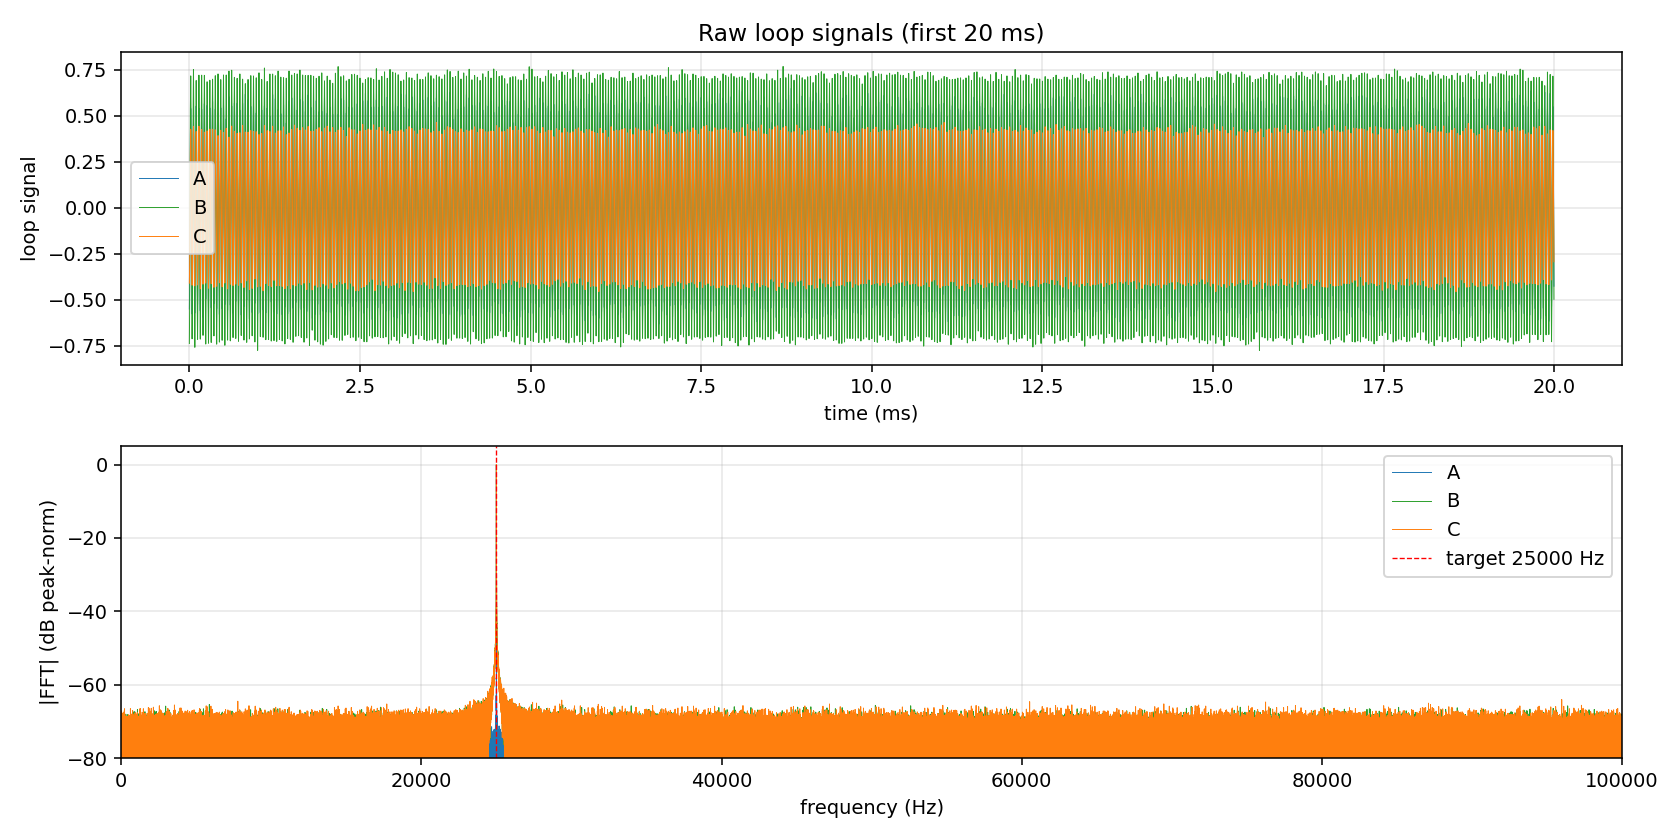
\includegraphics[width=0.95\linewidth]{figures/demo_linear_raw_spectra.png}
\caption{Raw three-loop signals (top) and per-loop FFT power spectra
(bottom) for the linear-pol simulated capture.  The dashed red line
marks the requested carrier (25\,kHz); the spectral peak is clearly
visible above the noise floor on all three loops, with channel-to-channel
amplitude ratios consistent with the cube-vertex projection of a
single linear polarization.}
\label{fig:linear-spectra}
\end{figure}

\begin{figure}[h]\centering
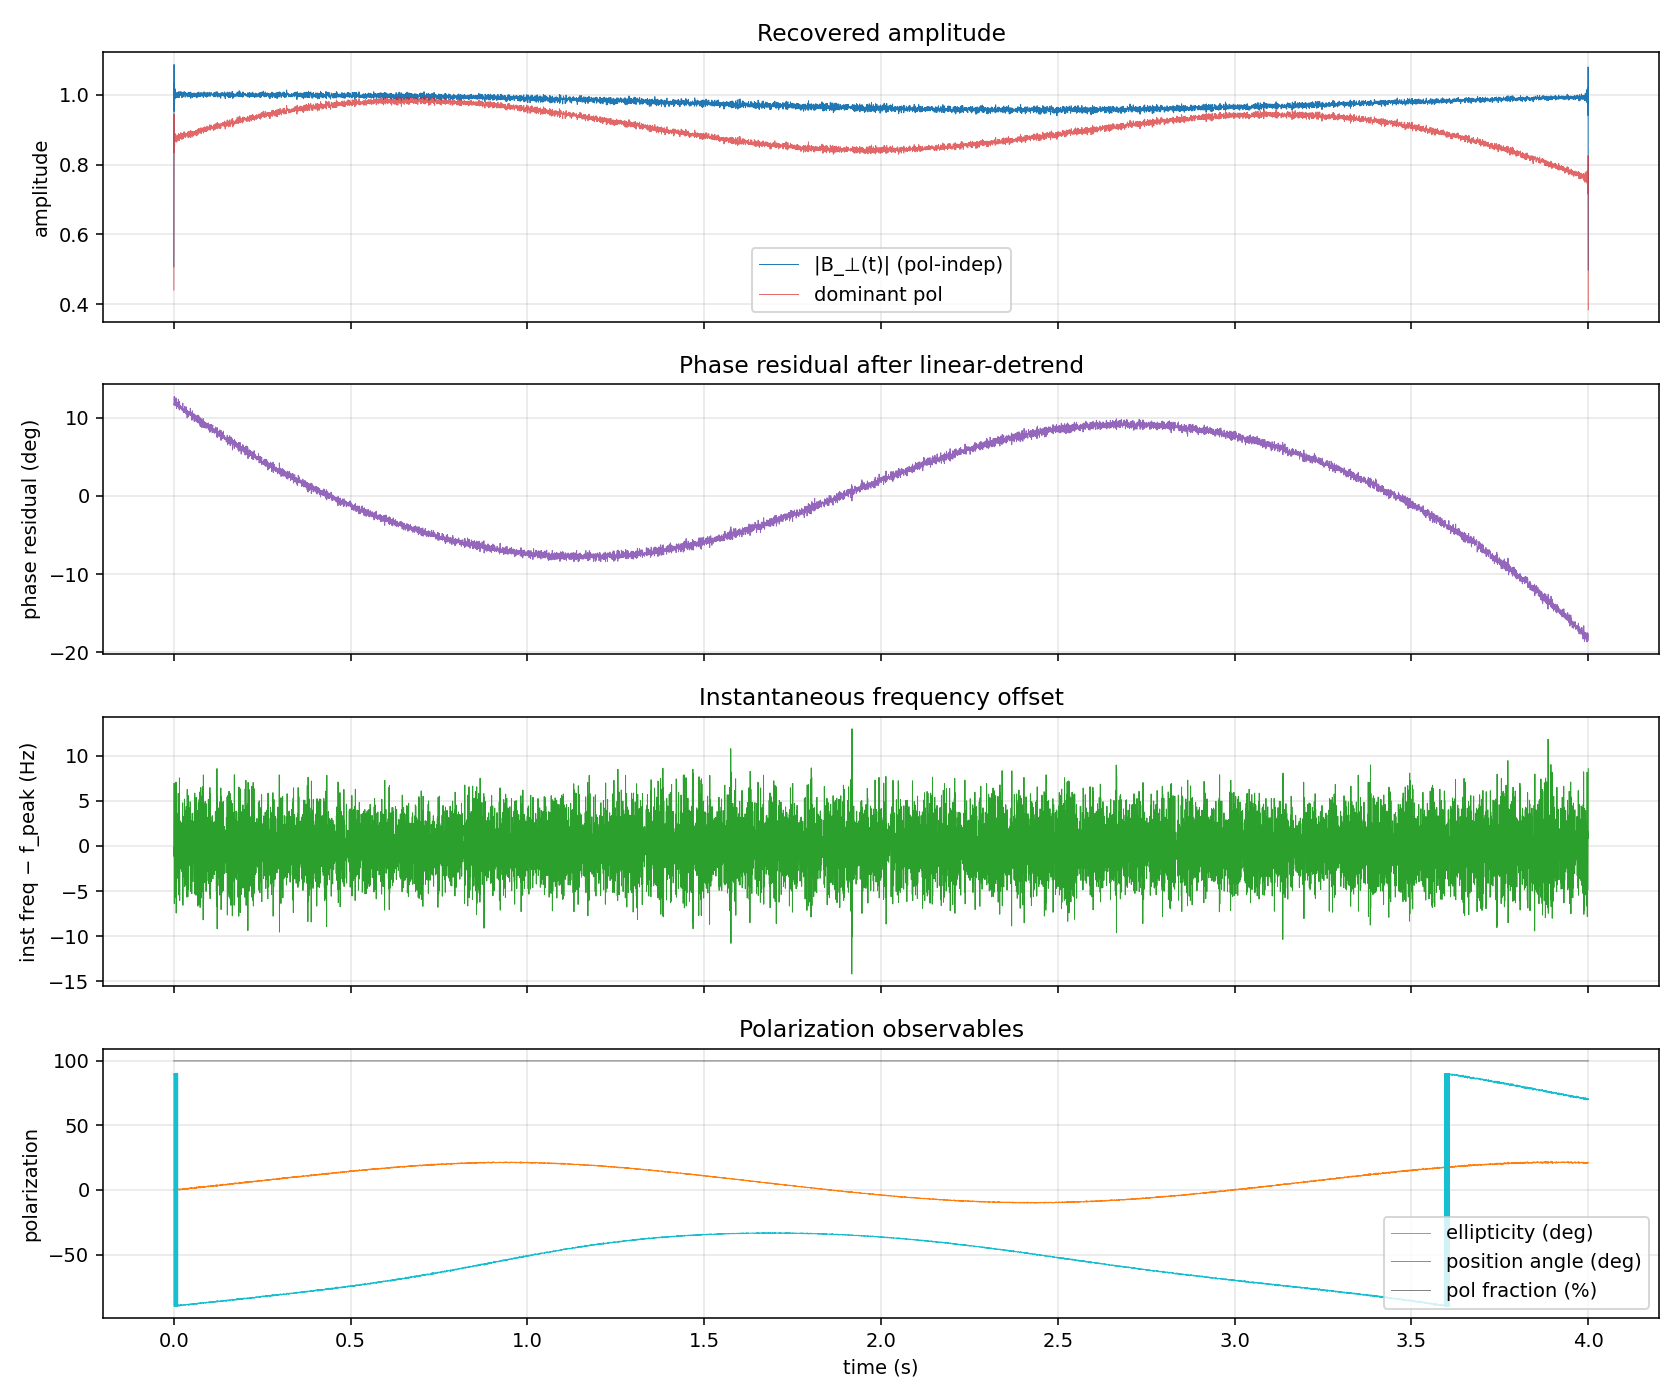
\includegraphics[width=0.95\linewidth]{figures/demo_linear_diagnostics.png}
\caption{Diagnostics for the linear-pol capture.  Top: the
polarization-independent intensity $|\mathbf B_\perp(t)|$ is
constant in time (Faraday rotation does not change wave intensity), but
the dominant-pol amplitude shows the characteristic Faraday fading.
Second: residual phase after linear detrending --- bounded and small.
Third: instantaneous frequency offset hovers near zero.  Fourth: the
position angle sweeps cleanly at $30^\circ$/s while ellipticity stays
near $0^\circ$ and polarization fraction stays at 100\,\%.}
\label{fig:linear-diag}
\end{figure}

\begin{figure}[h]\centering
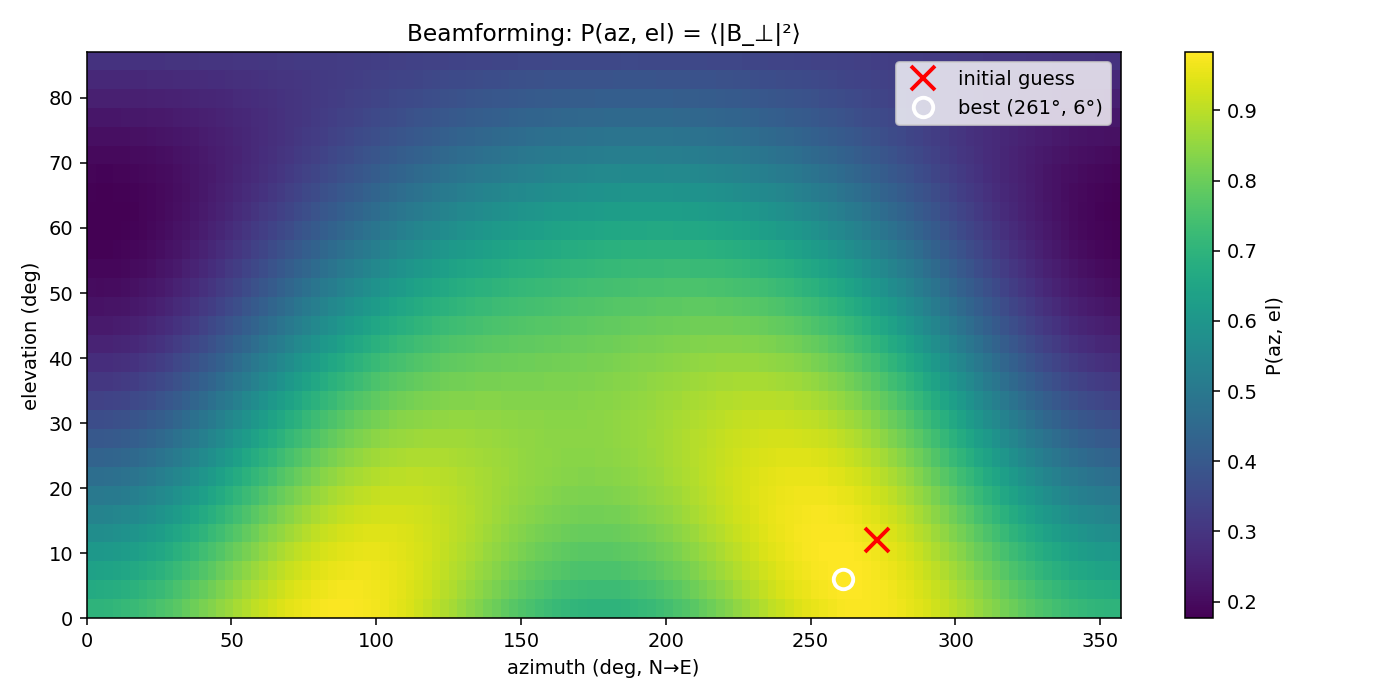
\includegraphics[width=0.85\linewidth]{figures/demo_linear_beamform.png}
\caption{Beamforming sweep $P(\varphi,\theta) = \langle |\mathbf
B_\perp|^2\rangle$ for the linear-pol capture.  The
red \texttt{x} marks the initial guess (273\textdegree, 12\textdegree);
the white circle marks the best-fit direction.  Note the
$\varphi\!\to\!\varphi+180^\circ$ ambiguity inherent to a single-point
B-vector array.}
\label{fig:linear-beam}
\end{figure}

\subsection{Example 2: right-circular polarization (the Faraday-immune control)}

For \emph{circularly} polarized input, Faraday rotation only adds a
common phase --- the wave's amplitude is unaffected.  A useful sanity
check on the pipeline:

\begin{lstlisting}[style=shell]
triloop simulate cap_rcp.h5 --pol rcp --faraday 30 --snr 25 --duration 4
triloop analyze cap_rcp.h5 --carrier 25000 --bw 2000 --az 273 --el 12
\end{lstlisting}

The analysis returns ellipticity $\approx -45^\circ$ (RCP) and
\emph{constant} amplitude in both the polarization-independent and
dominant-pol traces.

\begin{figure}[h]\centering
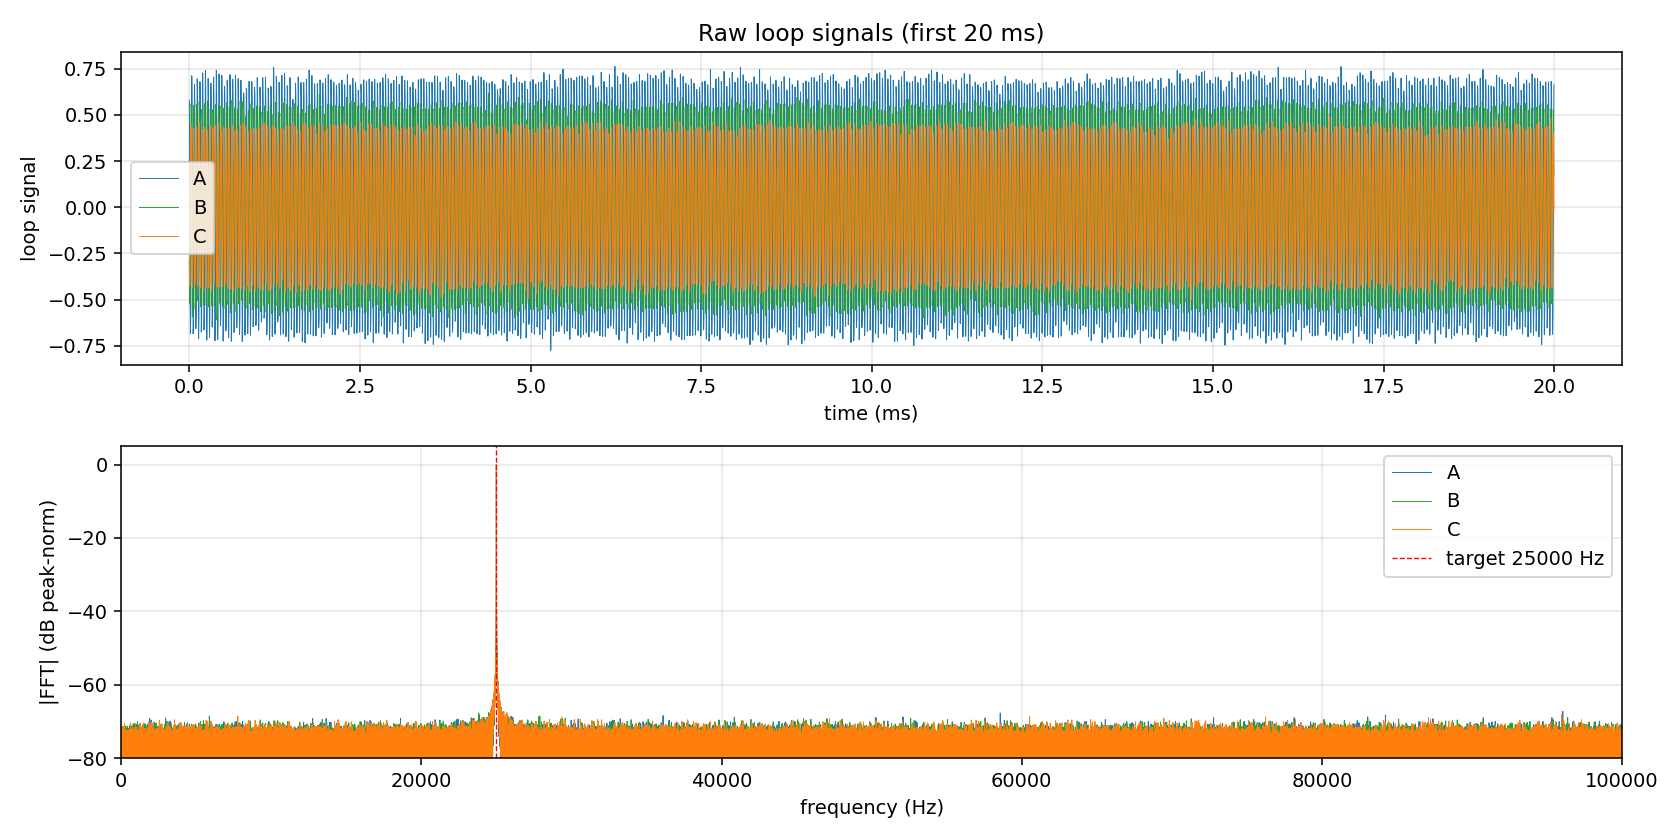
\includegraphics[width=0.95\linewidth]{figures/demo_rcp_raw_spectra.png}
\caption{Raw signals and spectra for the RCP capture.  All three loops
see the same carrier with comparable amplitudes (the RCP wave's
projection onto each loop is constant in magnitude up to a phase).}
\label{fig:rcp-spectra}
\end{figure}

\begin{figure}[h]\centering
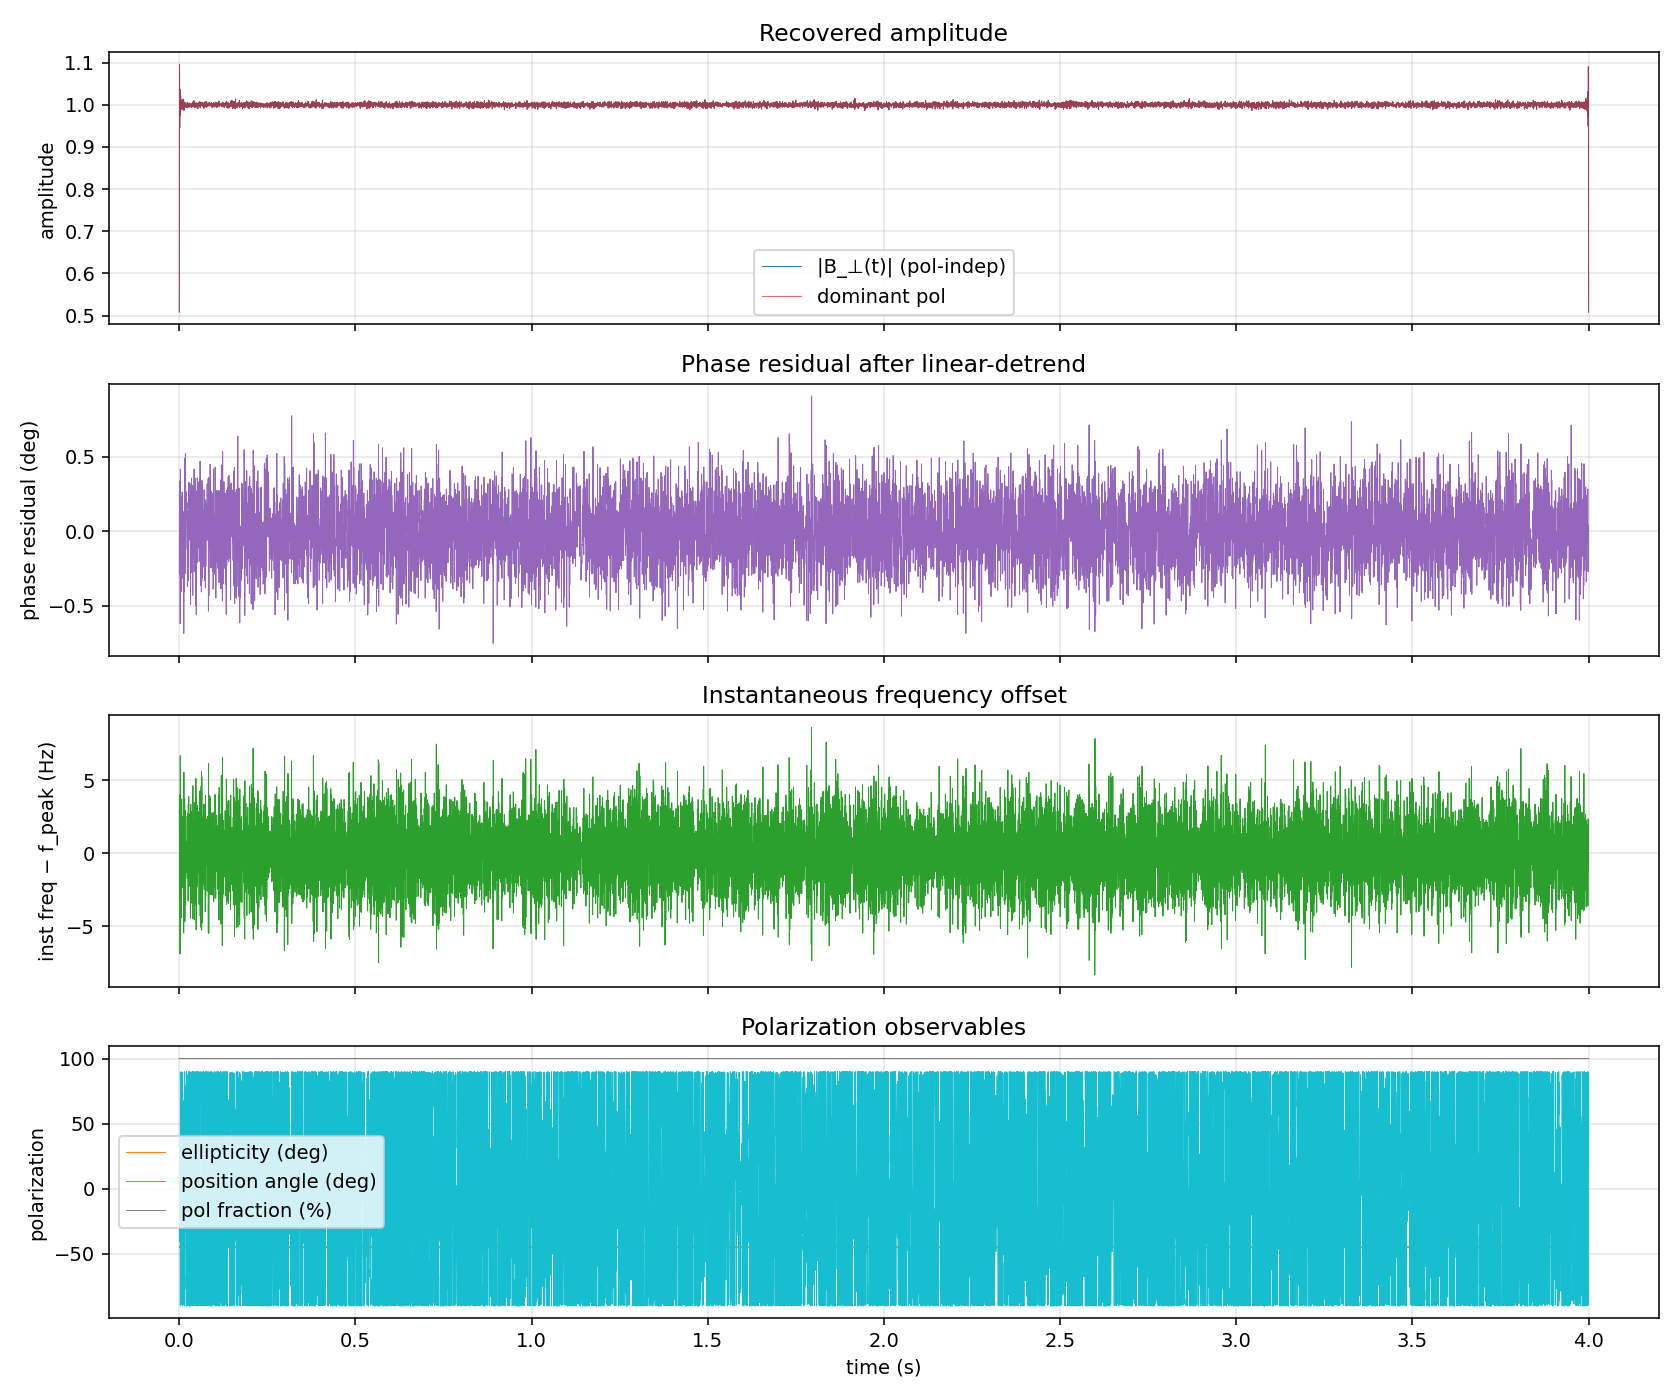
\includegraphics[width=0.95\linewidth]{figures/demo_rcp_diagnostics.png}
\caption{Diagnostics for the RCP capture.  Both the polarization-independent
intensity \emph{and} the dominant-pol amplitude are flat: Faraday rotation
of a circularly polarized wave is invisible to a magnitude-based
estimator.  Ellipticity sits at $\sim\!-45^\circ$ throughout.  The
position-angle estimator is meaningless for circular polarization (no
preferred linear axis) and consequently noisy.}
\label{fig:rcp-diag}
\end{figure}

\begin{figure}[h]\centering
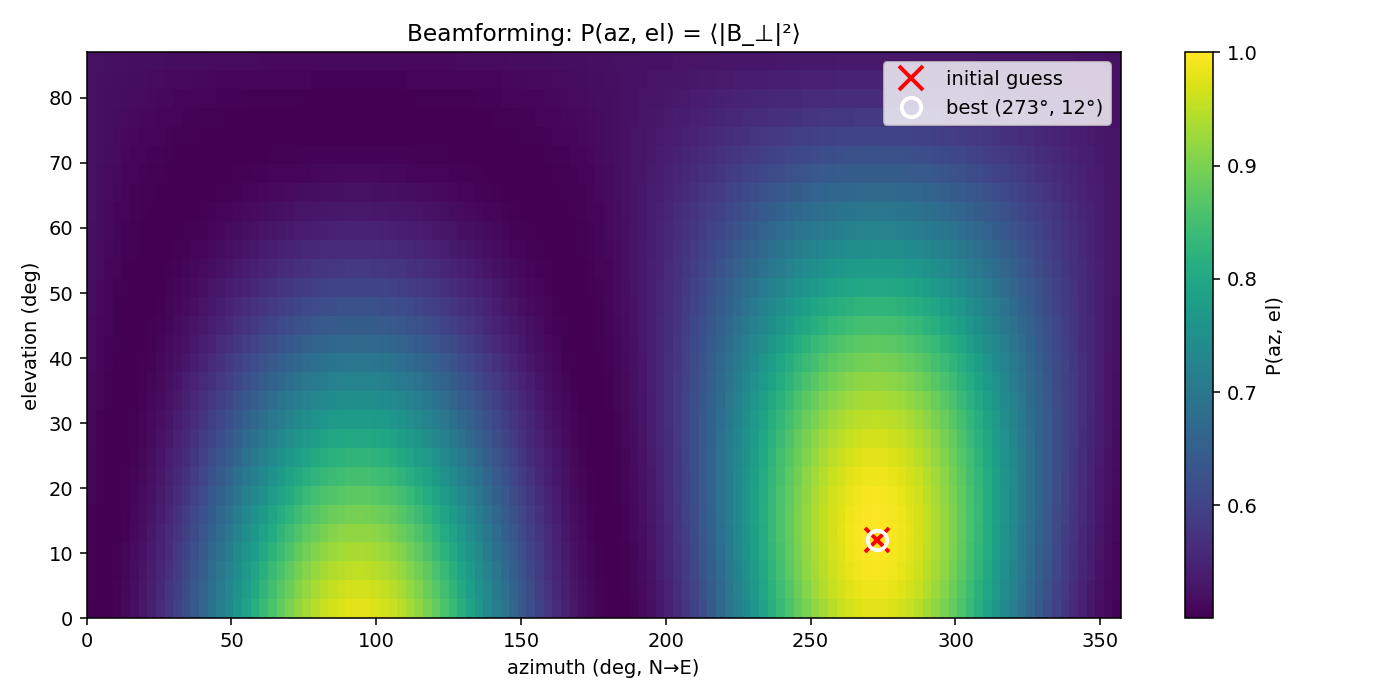
\includegraphics[width=0.85\linewidth]{figures/demo_rcp_beamform.png}
\caption{Beamforming sweep for the RCP capture.  Direction recovery is
unaffected by polarization state, as expected --- the
$|\mathbf B_\perp|^2$ estimator is intrinsically polarization-agnostic.}
\label{fig:rcp-beam}
\end{figure}

%-----------------------------------------------------------------------
\section{Python API reference}
%-----------------------------------------------------------------------

\subsection{Top-level functions}

\begin{lstlisting}[style=py]
from triloop import (
    read_capture, write_capture,
    analyze, analyze_z_loops, AnalysisResult,
    extract_bands, BandExtraction,
    analyze_all_bands, MultiBandResult, make_multiband_figure,
    make_view_figure,
    beamform_grid,
    estimate_direction_from_z_lab,
    null_search, perp_residual_energy, parabolic_refine,
    lock_and_analyze,
    default_loops_config,
    az_el_to_khat, perp_projector, perp_orthonormal_basis,
    extract_complex_baseband,
    compute_stokes,
)
# (the interactive browser builder lives in a submodule:)
from triloop.browse import build_browser_html, write_browser
\end{lstlisting}

\paragraph{\texttt{read\_capture(path) -> dict}}\quad\\
Read a triloop HDF5 file.  Returns a dict with keys
\texttt{sample\_rate, duration\_s, start\_time\_utc, scope\_model,
scope\_serial, capture\_settings, loops\_config, channels,
channel\_raw, time, format\_version}.

\paragraph{\texttt{write\_capture(path, channels, sample\_rate, ...)}}\quad\\
Write a triloop HDF5 file.  \texttt{channels} is a dict mapping
channel name to 1-D numpy array.  Optional kwargs include
\texttt{loops\_config}, \texttt{capture\_settings}, \texttt{scope\_model},
\texttt{scope\_serial}, \texttt{channel\_gains}, \texttt{channel\_offsets},
\texttt{store\_time\_array} (default \texttt{False}: regenerate $t$ from rate),
\texttt{compress} (default \texttt{True}: gzip level 4).

\paragraph{\texttt{analyze(t, B1, B2, B3, f0, BW, az\_deg, el\_deg, loops\_config=None) -> AnalysisResult}}\quad\\
Run the full pipeline.  Returns a dataclass with attributes:
\texttt{f\_peak, snr\_db\_per\_loop, z\_loops, z\_lab, z\_perp,
intensity, A\_p, A\_q, stokes\_I, stokes\_Q, stokes\_U, stokes\_V,
pol\_fraction, ellipticity\_deg, position\_angle\_deg, amp\_dominant,
instant\_phase, instant\_freq, instant\_freq\_mean,
khat, p\_hat, q\_hat, loops\_config, sample\_rate, duration\_s}.

\paragraph{\texttt{analyze\_z\_loops(t, Z\_loops, f\_peak, snrs\_db, az\_deg, el\_deg, loops\_config=None) -> AnalysisResult}}\quad\\
Same pipeline as \texttt{analyze}, but operates on a pre-extracted
complex-baseband array \texttt{Z\_loops} of shape (3, $N$) instead of
real-valued loop signals.  Used by the multi-band path so the FFT-based
mix/LPF only happens once per band rather than once per call.

\paragraph{\texttt{extract\_bands(cap, rf\_bands=None, bw\_hz=4000.0, decim\_rate\_hz=20000.0, channels=None) -> dict}}\quad\\
Multi-band complex-baseband extractor for bandpass-undersampled
captures.  For every \texttt{rf\_bands} entry (defaults to
\texttt{cap['capture\_settings']['rf\_bands\_hz']}) the function reads
the file's sample rate, computes the band's baseband alias position
via \texttt{picoacq.alias.alias\_of}, mixes-and-LPFs every selected
channel down, decimates to \texttt{decim\_rate\_hz}, and conjugates
even-Nyquist-zone slices so the analysis sees the spectrum the right
way around.  Returns a dict mapping \texttt{rf\_hz} (float) to a
\texttt{BandExtraction} dataclass with fields:
\texttt{rf\_hz, baseband\_hz, nyquist\_zone, inverted, bw\_hz,
decim\_rate\_hz, t, z} (where \texttt{z} is a dict mapping
channel name to \texttt{complex64} array).

\paragraph{\texttt{analyze\_all\_bands(cap, az\_deg, el\_deg, loops\_channels=("A","B","C"), bw\_hz=4000.0, decim\_rate\_hz=20000.0, rf\_bands=None, loops\_config=None) -> dict}}\quad\\
Convenience wrapper that calls \texttt{extract\_bands} and then
\texttt{analyze\_z\_loops} on each band.  Returns a dict mapping
\texttt{rf\_hz} to a \texttt{MultiBandResult}
(\texttt{rf\_hz, extraction, analysis, snrs\_db}).

\paragraph{\texttt{make\_multiband\_figure(results, out\_path=None)}}\quad\\
Build a Matplotlib figure with one row per band $\times$ four columns
(intensity, instantaneous frequency, ellipticity, polarization
fraction).  Either save to \texttt{out\_path} or return the figure
object.

\paragraph{\texttt{make\_view\_figure(cap, rf\_bands=None, bw\_hz=8000.0, out\_path=None)}}\quad\\
Build the static QC PNG used by the \texttt{view} subcommand.

\paragraph{\texttt{build\_browser\_html(cap, az\_deg=9, el\_deg=35, loops\_channels=("A","B","C"), bw\_hz=4000, decim\_rate\_hz=20000, n\_anim\_frames=60, title=None) -> str}}\quad\\
Return an HTML string containing the full interactive browser
(\textbf{Section~\ref{sec:browse}}).  The companion
\texttt{write\_browser(cap, out\_path, **kw)} writes it to disk.

\paragraph{\texttt{beamform\_grid(z\_loops, loops\_config, az\_grid\_deg=None, el\_grid\_deg=None) -> (P, az, el)}}\quad\\
Compute the time-averaged $P(\varphi,\theta)$ on a 2-D grid.

\paragraph{\texttt{extract\_complex\_baseband(t, b, f0, BW) -> (z, f\_peak, snr\_db)}}\quad\\
Find the spectral peak nearest to \texttt{f0} within $\pm\,$\texttt{BW}
in the real signal \texttt{b(t)}, mix to baseband, and brick-wall
low-pass to $\pm\,$\texttt{BW/2}.

\paragraph{\texttt{estimate\_direction\_from\_z\_lab(Z\_lab) -> dict}}\quad\\
Eigendecompose the lab-frame coherency matrix
$\mathsf{C} = \langle\mathbf z\mathbf z^H\rangle$ and return the
smallest-eigenvalue eigenvector as $\hat{\mathbf k}_{\rm est}$, its
$(\varphi,\theta)$, the eigenvalues (descending), the polarization
basis ($\hat{\mathbf p}$, $\hat{\mathbf q}$ from the two largest
eigenvectors), and a \texttt{null\_strength} $\lambda_3/\lambda_1$.

\paragraph{\texttt{null\_search(Z\_lab, az0, el0, half\_width\_deg, n\_points) -> dict}}\quad\\
2-D grid sweep around an initial guess that minimises
$\langle |\hat{\mathbf k}_{\rm trial}\cdot\mathbf z_{\rm lab}|^2\rangle$.
Returns the residual map and best-on-grid direction.

\paragraph{\texttt{lock\_and\_analyze(t, B1, B2, B3, f0, BW, az0=None, el0=None, ...) -> dict}}\quad\\
End-to-end direction-finding plus polarimetry: extract complex
baseband, eigendecompose, run the null sweep (optional), parabolic
sub-grid refinement, then perp-plane projection and Stokes
computation locked to the recovered direction.  See
Section~\ref{sec:locate}.

\subsection{Example: scripted analysis}

\begin{lstlisting}[style=py]
import numpy as np
from triloop import read_capture, analyze, beamform_grid

cap = read_capture("cap.h5")
B1, B2, B3 = cap["channels"]["A"], cap["channels"]["B"], cap["channels"]["C"]
res = analyze(cap["time"], B1, B2, B3,
              f0=25_000.0, BW=2000.0, az_deg=273.0, el_deg=12.0,
              loops_config=cap["loops_config"])

print(f"f_peak = {res.f_peak:.4f} Hz")
print(f"polarization fraction = {np.median(res.pol_fraction):.3f}")
print(f"ellipticity (deg) = {np.median(res.ellipticity_deg):+.2f}")

# beamform
P, az, el = beamform_grid(res.z_loops, cap["loops_config"])
i, j = np.unravel_index(np.argmax(P), P.shape)
print(f"best az,el = ({az[j]:.0f}, {el[i]:.0f})")
\end{lstlisting}

%-----------------------------------------------------------------------
\section{Calibration and known limitations}
%-----------------------------------------------------------------------

\subsection{Per-loop calibration is critical}

The analysis assumes the three loops have equal effective area, gain,
and phase response at the operating frequency.  Real loops never quite
do.  Without calibration, intensity estimates can be off by a few
\%, position angles by a few degrees, and ellipticity may be biased
away from $0^\circ$ even for nominally linear input.

The cleanest calibration procedure:

\begin{enumerate}\itemsep=2pt
\item Transmit a known-direction CW signal of known polarization
      (e.g.\ a vertically polarized test transmitter at a known site).
\item Capture with \texttt{picoacq capture}.
\item Compare the analysis output's recovered position angle and
      ellipticity to ground truth.
\item Solve for per-loop \texttt{gain} and \texttt{phase\_offset\_deg}
      that drive the recovered values to ground truth, and store them
      in the \texttt{loops\_config} for production use.
\end{enumerate}

\subsection{Front/back ambiguity}

A single-point three-loop B-field array is symmetric under
$\hat{\mathbf k}\to -\hat{\mathbf k}$: the beamforming map satisfies
$P(\varphi,\theta) = P(\varphi+180^\circ, -\theta)$.  This is intrinsic
geometry, not a software bug; resolving it requires either an
additional E-field probe or a phased pair of triplets.

\subsection{Coherent sampling}

\textsf{triloop} requires that the three loops be sampled with a
shared LO and ADC clock --- i.e.\ a single multi-channel digitiser like
the PicoScope 5444D, NOT three independent KiwiSDRs.  Without
coherent sampling, channel-to-channel phase information is corrupted
by independent oscillator drift, and Stokes parameters become
unrecoverable.

\subsection{SNR gain over a naïve power sum}

For an \emph{isotropic noise} background and the cube-vertex geometry,
the coherent direction-formed estimator $|\mathbf{B}_\perp(\hat{\mathbf k})|^2$
achieves an SNR exactly $3/2$ ($+1.76$\,dB) higher than incoherently
summing the three loop powers $\sum_i |B_i|^2$, regardless of the
source direction.  Two ingredients give this result: the cube-vertex
loop normals form a tight frame ($\sum_i \hat{\mathbf n}_i\hat{\mathbf n}_i^{\!\top}\!=\!\mathsf{I}$),
which makes the loop-frame noise transformation to lab frame exactly
isotropic; and projecting onto the plane perpendicular to $\hat{\mathbf k}$
removes one of three orthogonal noise dimensions while preserving the
full signal (which lives in that perpendicular plane by construction).
The gain is $+1.76$\,dB at every $(\varphi,\theta)$.

\subsection{Single-point direction finding is impossible for purely
linearly polarized signals}
\label{sec:rank1}

A single linearly-polarized plane wave produces a \emph{rank-1}
coherency matrix
$\mathsf{C} = \langle\mathbf{z}_{\mathrm{lab}}\mathbf{z}_{\mathrm{lab}}^H\rangle$
--- only one eigenvalue is non-zero, and the corresponding eigenvector
points along the polarization, not along $\hat{\mathbf k}$.  The two
remaining eigenvalues are degenerate at zero (in the noise-free
limit), so the smallest-eigenvalue eigenvector --- which we use to
estimate $\hat{\mathbf k}$ --- is ambiguous in any direction within
the 2-D plane perpendicular to $\hat{\mathbf{e}}_{\rm pol}$.

Equivalently: the perp-residual energy
$\langle |\hat{\mathbf k}_{\mathrm{trial}}\cdot\mathbf B(t)|^2\rangle$
is zero whenever $\hat{\mathbf k}_{\mathrm{trial}} \perp
\hat{\mathbf{e}}_{\rm pol}$, not just when $\hat{\mathbf k}_{\mathrm{trial}}
=\pm\hat{\mathbf k}_{\rm true}$.  The null is a plane, not a point.

To direction-find a linearly polarized signal from a single 3-loop
station you must break the rank-1 condition by introducing a second
linearly-independent polarization sample.  Three options work in
practice:

\begin{itemize}\itemsep=2pt
\item \textbf{Faraday rotation:} if the propagation path imprints a
      time-varying polarization rotation, the polarization axis
      sweeps through a range of angles during the integration time
      and the time-averaged coherency becomes rank-2.  At HF this
      happens naturally on most ionospheric paths, especially at
      lower frequencies where Faraday is large.
\item \textbf{Circularly polarized source.}  RCP and LCP are
      intrinsically rank-2: the perp-plane is filled both by
      $\hat{\mathbf p}$ and $\hat{\mathbf q}$.  The null eigenvector
      is unambiguous.
\item \textbf{Triangulation.}  Two spatially separated three-loop
      stations resolve the ambiguity, because the rank-1 plane is
      different at each station and they intersect along
      $\hat{\mathbf k}_{\rm true}$.
\end{itemize}

The eigendecomposition reports a small but \emph{non}-zero
\texttt{null\_strength} ($\lambda_3/\lambda_1$) when the rank-1
condition is broken in any of these ways.  When
\texttt{null\_strength} is small, the direction estimate is
trustworthy.  When it approaches the ratio of the second-smallest to
largest eigenvalue (i.e.\ the rank-1 nullspace is degenerate), trust
the result only after polarization diversity has been confirmed.

\subsection{Beam pattern is broad}

The polarization-independent estimator $|\mathbf B_\perp|^2$ has a
$\frac{1}{2}+\frac{1}{2}\cos^2\!\beta$ angular pattern relative to
$\hat{\mathbf k}_\mathrm{target}$.  This is a \emph{factor of two}
between on-axis and broadside, not a sharp pencil beam.  Direction
finding via beamforming is therefore approximate; for the cleanest
direction estimate, eigendecompose $\langle z_iz_j^*\rangle$ and read
off the smallest-eigenvalue eigenvector --- this is implemented in
upcoming versions.

%-----------------------------------------------------------------------
\section{Appendix: file layout in the source tree}
%-----------------------------------------------------------------------

\begin{lstlisting}[style=shell]
triloop/                           analysis package
  pyproject.toml
  README.md
  triloop/
    __init__.py
    geometry.py        -- N matrix, projector, p-hat / q-hat basis
    extract.py         -- narrow-band complex baseband (single tone)
    bands.py           -- multi-band extraction (calls picoacq.alias)
    stokes.py          -- Stokes parameters from (A_p, A_q)
    analyze.py         -- analyze() + analyze_z_loops() + AnalysisResult
    multiband.py       -- analyze_all_bands(), make_multiband_figure()
    direction.py       -- null-eigenvector + null-sweep direction finding
    beamform.py        -- P(az, el) sweep
    view.py            -- static QC PNG (matplotlib)
    browse.py          -- interactive HTML browser (Plotly)
    io_hdf5.py         -- HDF5 reader / writer
    config.py          -- loops_config dict + validator
    cli.py             -- click-based command-line interface
  notebooks/
    triloop_analysis.ipynb
  tests/
    test_simulated_recovery.py
  docs/
    triloop_user_manual.tex      (this file)
    triloop_analysis_ref.tex     (developer's reference)
    figures/

picoacq/                           acquisition package
  pyproject.toml
  README.md
  picoacq/
    __init__.py
    ps5444a.py         -- thin PicoSDK 5000a wrapper
    simulator.py       -- no-hardware fallback
    recorder.py        -- capture orchestrator + onboard-buffer guard
    alias.py           -- bandpass-undersampling alias map (RF<->baseband)
    cli.py             -- click-based CLI (capture + monitor)
  docs/
    picoacq_user_manual.tex
\end{lstlisting}

\end{document}
